\chapter{Conclusion and Future Work}
\label{chap:conclusion}

\section{Summary of Achievements Against Objectives}

This graduation project designed, implemented, and empirically evaluated \textbf{CITRA} (\textit{Essay Integrity Checker v3.90.6}), an explainable neuro-symbolic software platform for automated Citation Integrity Scoring (CIS), fabricated reference detection, and bibliography remediation. Table~\ref{tab:obj-summary} maps the delivered software artifacts and empirical results directly back to the six research objectives defined in Section~\ref{sec:objectives}.

{\setlength{\tabcolsep}{3.5pt}
\begin{longtable}{|C{0.14}|L{0.32}|L{0.54}|}
\caption{Summary of graduation project achievements mapped against project research objectives.}\label{tab:obj-summary}\\
\hline
\textbf{Objective} & \textbf{Target Capability} & \textbf{Delivered Engineering \& Empirical Outcome} \\
\hline
\endfirsthead
\multicolumn{3}{c}{\itshape Table \thetable\ (continued from previous page)}\\
\hline
\textbf{Objective} & \textbf{Target Capability} & \textbf{Delivered Engineering \& Empirical Outcome} \\
\hline
\endhead
\hline
\multicolumn{3}{r}{\itshape Continued on next page}\\
\endfoot
\hline
\endlastfoot
\textbf{OBJ-1} & \textbf{Multi-format extraction \& bidirectional linking} & Hybrid GROBID \texttt{0.9.1-crf} TEI-XML + PyMuPDF + \texttt{python-docx} across \textbf{12 styles} (incl.\ VN laws) and 7-method linker (\textbf{$97.7\%$--$100\%$} bib.\ detection on 310 PDFs). \\
\hline
\textbf{OBJ-2} & \textbf{Domain-aware federated retrieval} & \textbf{129,137-record} SQLite FTS5 corpus (\textbf{$99.80\%$} recall, $87.6\text{\,ms}$) + \textbf{15+ live APIs}, Retraction Watch, singleflight cache, and pinned-IP URL/HTML validators. \\
\hline
\textbf{OBJ-3} & \textbf{Neuro-symbolic verification \& calibration} & Dual SBERT + ONNX INT8 \texttt{VI}$\leftrightarrow$\texttt{EN} encoders fused with \textbf{68 symbolic rules}, 16D MLR ($C=0.25$), and Platt scaling (\textbf{$\text{ECE} = 0.0411$}, \textbf{$\text{Brier} = 0.0108$}). \\
\hline
\textbf{OBJ-4} & \textbf{Interpretable CIS grading \& remediation} & Five-component CIS rubric (\textbf{$\rho = 0.9987$} rank stability) plus automated APA, IEEE, TDTU, BibTeX, RIS, and \texttt{.docx} bibliography repair. \\
\hline
\textbf{OBJ-5} & \textbf{Secure role-based web platform} & Containerized FastAPI (\textbf{15 ORM tables}, 13 migrations (\texttt{0001}--\texttt{0013}), SSE, RBAC/IDOR, pinned-IP SSRF defense) \& React 18.3 SPA (\textbf{$228.42\text{\,kB}$} entry). \\
\hline
\textbf{OBJ-6} & \textbf{Leak-free large-scale evaluation} & \textbf{$99.20\%$} ID accuracy ($N=18\text{K}$), \textbf{$99.96\%$} OOD accuracy ($N=2.4\text{K}$), \textbf{$100\%$} 6-domain E2E accuracy ($120/120$), and \textbf{$50/50$} burst concurrency. \\
\hline
\end{longtable}
}

Figure~\ref{fig:verdict-paths} synthesizes the core architectural safeguard governing every verdict in \textbf{CITRA}: substantive accusations (\texttt{suspected\_hallucination}) require either positive structural refutation (fabricated/chimeric DOI, RFC 2606 fake domain, impossible future year) or clean HTTP 200 empty responses across multiple live registries, whereas network exhaustion, unindexed regional DOIs, and borderline similarities ($[0.40, 0.60)$) route deterministically to \texttt{unresolved} for human review.

\begin{figure}[H]
    \centering
    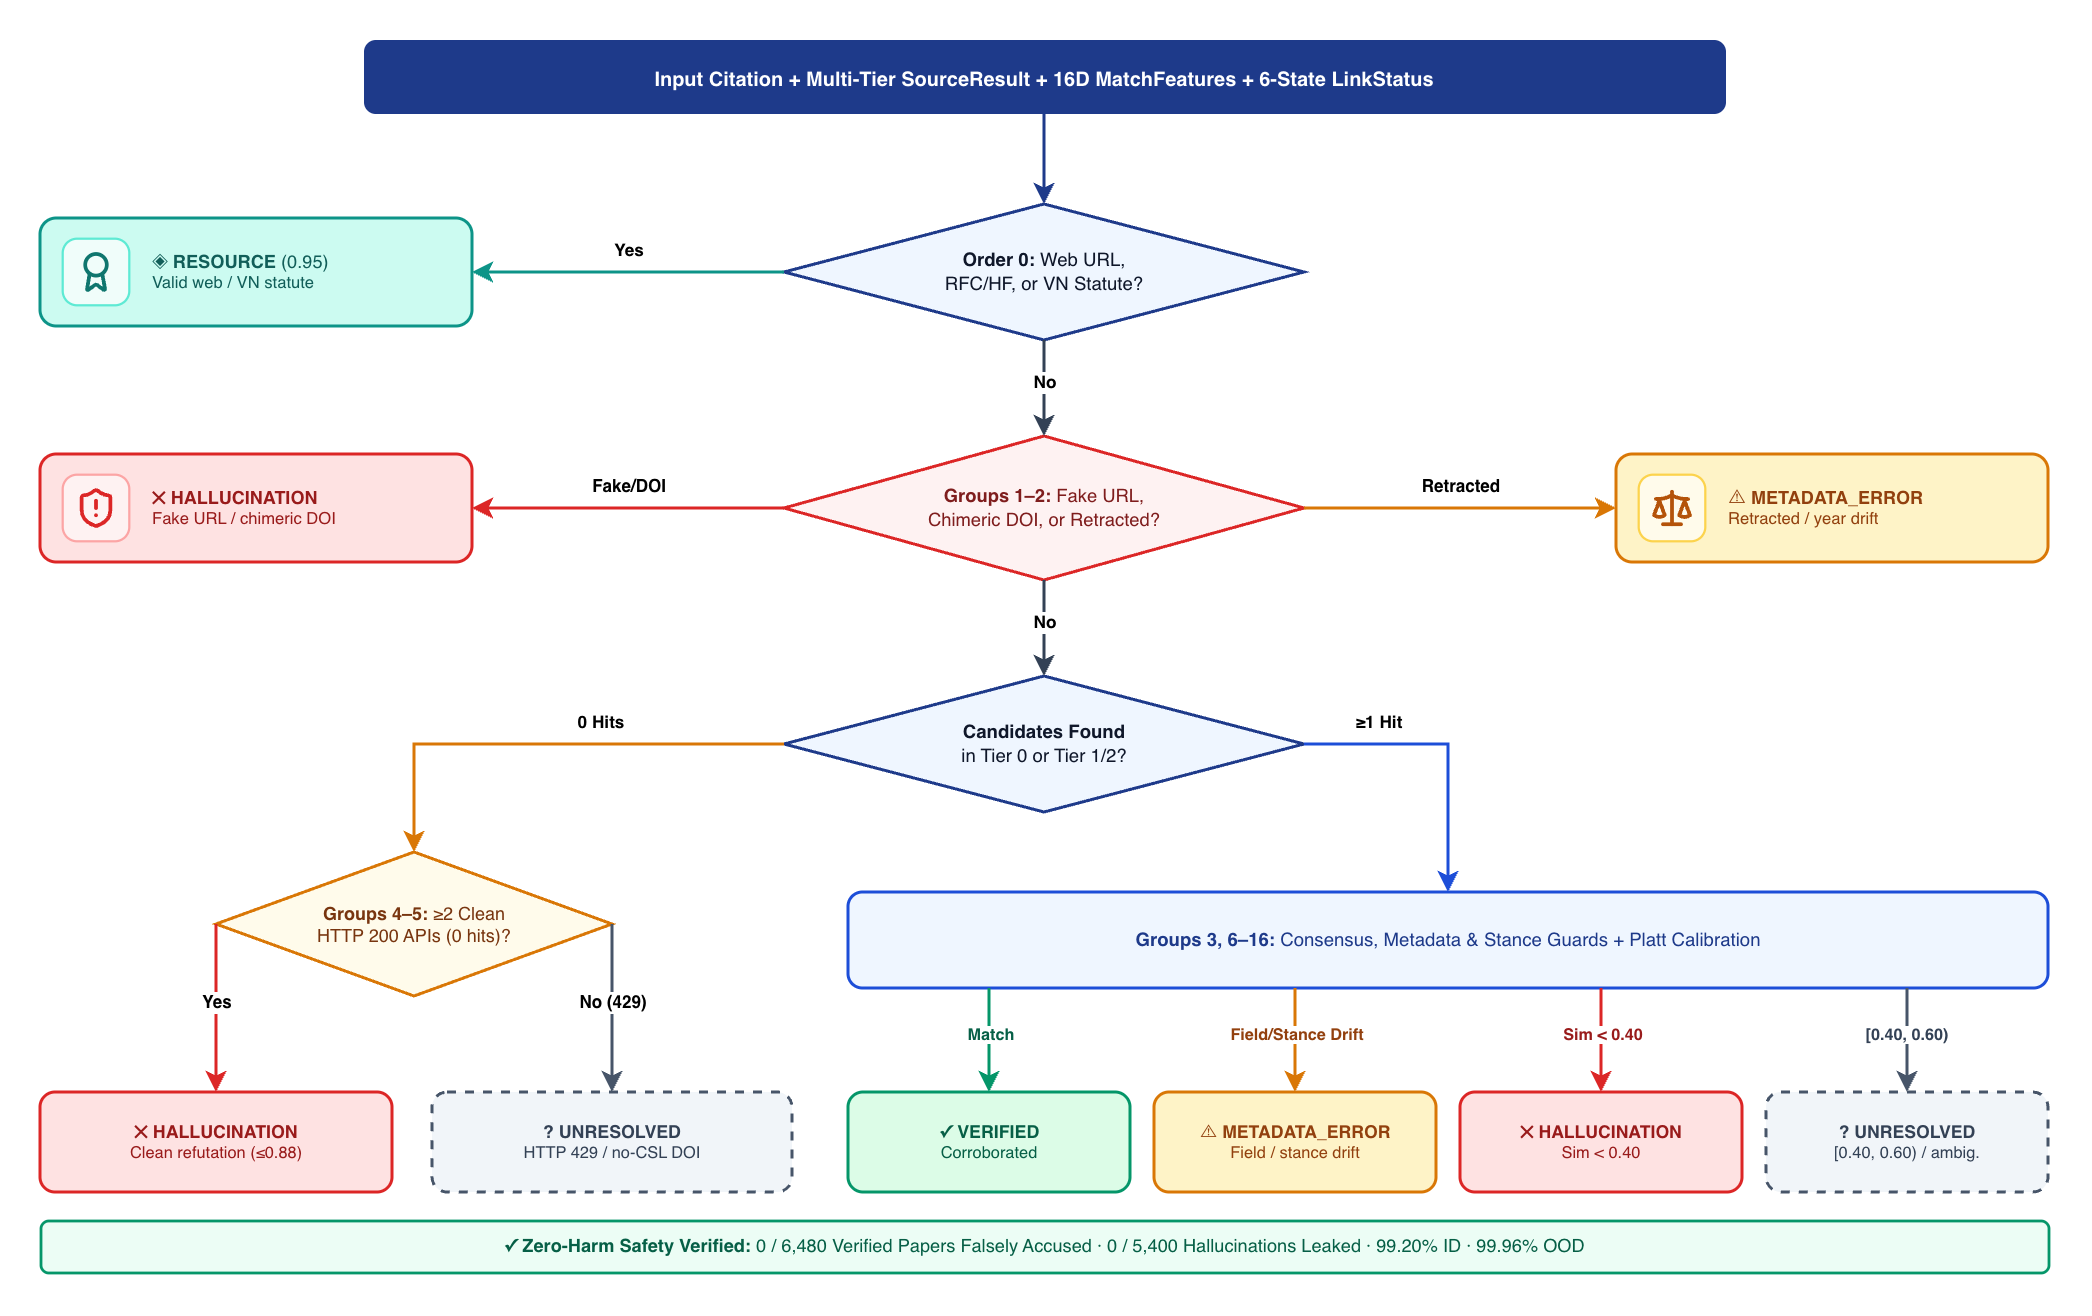
\includegraphics[width=\textwidth,keepaspectratio]{picture/figures/fig6_1_verdict_paths.png}
    \caption[Guarded neuro-symbolic decision tree separating refutation from abstention]{Guarded neuro-symbolic decision tree in CITRA (\texttt{v3.90.6}) separating evidence-backed refutation (\texttt{suspected\_hallucination}) from provenance-aware abstention (\texttt{unresolved}).}
    \label{fig:verdict-paths}
\end{figure}

\section{Synthesis of Key Empirical Findings}

Three empirical lessons emerge from the experiments in Chapter~\ref{chap:results}:
\begin{enumerate}
    \item \textbf{Symbolic rules and statistical learning are complementary, not redundant.} Pure 16-dimensional Logistic Regression (\texttt{B5}) performs well on smooth similarity trade-offs ($97.67\%$ ID) yet collapses to $57.37\%$ on discrete OOD integrity rules (such as retracted articles, fake URLs, or Vietnamese statutory authority mismatches). Combining priority-ordered symbolic guardrails with ML probability blending achieves both $99.20\%$ ID accuracy and $99.96\%$ OOD accuracy.
    \item \textbf{Post-hoc calibration is essential for trustworthy confidence reporting.} Raw symbolic rule confidences suffer from severe overconfidence ($\text{ECE} = 0.2475$). Logit-space Platt scaling lowers ECE by $6.02\times$ to $0.0411$ and Brier Score by $8.38\times$ to $0.0108$ while preserving exact non-abstention coverage ($87.83\%$).
    \item \textbf{Offline FTS5 indexing makes CPU-only classroom deployment practical.} Caching verified candidates and indexing 129,137 papers locally yields a $688.72\times$ retrieval speedup and allows a single CPU server to handle 50 simultaneous deadline uploads without external rate-limit collapse.
\end{enumerate}

\section{System Limitations}
\label{sec:limitations}

Despite strong empirical performance, version \texttt{3.90.6} has four concrete engineering limitations:
\begin{itemize}
    \item \textbf{L1 (Paywalled Full-Text Claim Blindness):} Semantic claim alignment compares inline sentences against titles and open abstracts. When a student cites a specific figure, theorem, or discussion paragraph inside a closed-access article whose abstract omits that detail, \textbf{CITRA} cannot verify body-level entailment.
    \item \textbf{L2 (Domain Skew in the Offline Corpus):} Because $98.42\%$ of \texttt{local\_papers.db} originates from the ACL Anthology and CS arXiv, fully air-gapped deployments without Internet access experience reduced Tier-0 recall on biomedical, humanities, and Vietnamese domestic journal articles.
    \item \textbf{L3 (Complex Multi-Column Archival and Handwritten Scans):} Although selective Tesseract OCR recovers printed Vietnamese pages, low-resolution camera scans, skewed archival manuscripts, and handwritten margin citations degrade character accuracy and increase \texttt{unresolved} rates.
    \item \textbf{L4 (Single-Host SQLite Write Serialization):} While SQLite WAL handles 50 concurrent student uploads on a single host, scaling horizontally across multiple independent API virtual machines requires a network-shared relational database and distributed message broker.
\end{itemize}

\section{Future Work}
\label{sec:future-work}

Each limitation in Section~\ref{sec:limitations} motivates a direct future engineering direction:
\begin{itemize}
    \item \textbf{F1 (Open-Access Full-Text Passage Retrieval $\leftarrow$ L1):} Integrate PubMed Central JATS XML, arXiv HTML5 (\texttt{ar5iv}), and Unpaywall open-access PDFs with paragraph-level dense passage retrieval so claim verification extends beyond abstracts whenever open licenses permit.
    \item \textbf{F2 (Multidisciplinary and ASEAN Offline Corpus Expansion $\leftarrow$ L2):} Expand \texttt{local\_papers.db} with open snapshots from DOAJ, Vietnam Journals Online (VJOL), and OpenAlex subfield slices to provide balanced offline coverage across economics, law, biomedicine, and engineering.
    \item \textbf{F3 (Layout-Aware Vision-Language OCR $\leftarrow$ L3):} Incorporate lightweight CPU-quantized document layout models (such as Docling or Surya OCR) to improve reference segmentation on degraded archival scans and complex footnote-heavy humanities manuscripts.
    \item \textbf{F4 (PostgreSQL + Redis Worker Scaling and LTI 1.3 LMS Integration $\leftarrow$ L4):} Support optional PostgreSQL connection pooling and Redis task queues alongside Learning Tools Interoperability (LTI 1.3) webhooks for Moodle and Canvas gradebooks, enabling multi-faculty longitudinal studies across semesters.
\end{itemize}

\section{Concluding Remarks}

Software tools used in academic assessment carry an obligation of fairness and transparency. By grounding every citation check in traceable external registries, combining neural semantic alignment with 68 auditable symbolic rules and Platt-calibrated probabilities, abstaining honestly when evidence is incomplete, and placing final override authority in the hands of instructors, \textbf{CITRA} demonstrates a practical software engineering blueprint for trustworthy AI-assisted academic integrity verification.
